

\section{Discovering Povodni Mož}

\margininbox{Povodni Mož}{
     \begin{itemize}
    \item Erik Bončina
    \item Nejc Maver
    \item Izi Možir
    \item Tjaša Rutar
    \end{itemize}}{\explo}

After couple of days on the surface, I decided to do some camping with
my Slovenian mates. Tjaša, Erik, Mawer and I started to walk towards the
entrance of \passage{Vrtnarija} at around 2 am. We reached the camp too
early for our bed time
\sidenote{On the Night Train, the bed time is 8 am to 8 pm}, so we
decided to go and check out the crystals in \passage{Palace of King Minos}.
After this, we still had time so we decided to go and try digging in
\passage{Minotaur Rift}, where last time with Dan we could hear the
enticing `roar' of water. After couple of hours moving boulders with no
breakthrough, we returned to camp.


The next day we planned to investigate one lead in \passage{Palace of King
Minos}, that we had not yet pushed with Dan. The entrance to the lead
was quite narrow, but beyond it we reached a series of active water
pitches. We had enough rope to bolt two drops and decided to name the
passage \passage{Povodni mož} \sidenote{Water nymph}, as we had been
following the water all the time.

\name{Izi Možir}

\subsection{Continuing to explore Povodni mož: the story from the underground logbook}

\textbf{6-8-10 23:48}

Back again for my seventh night! Fratnik and I had a smooth 2hr journey
down. Met Nicholas and Thara just about to head out. Jarv and Myles are
here too (soon to go down \passage{Korita}). James and William then turned up. TEA
all round! Fratnik and I eventually went for a tourist jolly to the
\passage{Queen's Bed Chamber}. Then we went down to push \passage{Povodni Mož}. Wow! A small
hole in a large dry passage soon leads to small fossil stream passage
then to nice active stream. Went down 2 pitches (pushed by Izi, Erik,
Tjaša and Mawr). Bagged one more then half bolted another. Back to camp
for tea (and medals). It's clearly raining outside -- \passage{Zimmer} is
very wet. Hope Jarv and Myles (now back from pushing \passage{Korita}) make it out
OK!

\name{Tetley}

\margininbox{6-8-10}{
Jarv and Myles. Train crash! Having rotated onto the day-train we
collided with Tet, Fratnik, JKP and William. So we must away, a long way
to the bivi, at least, when you leave at two minutes to midnight\ldots{}
\passage{Korita} is dead, without explosive. Derigged entirely to the
3\textsuperscript{rd} pitch. \name{Jarv}}{\logbook}

\textbf{7-8-10 9:50 a.m.}

Tea cooling down\ldots{} Fratnik is making food, James is putting his
wetish furry on, \textit{Dirty Old Town }playing on sterio.
\name{Tetley}

\textbf{7-8-10 11:10 a.m.}

Final hot vitaminski -- then James and William to \passage{Serpentine}, Tetley and Fratnik to \passage{Povodni Mož}. `Dangerous Dick' is seeping slowly into my subconscious\ldots{}

\name{Tetley}

\newpage
\textbf{7-8-10 11:15 p.m.}

Fratnik and I are back and well fed. A great days caving. Sadly \passage{Povodni Mož} is now dead: Upstream pushed to 30 m+ aven; bolting downstream, we eventually hit a sump. All now surveyed and derigged. Now time for bed.

\name{Tetley}

\textbf{8.8.10}

Drugo leto spet, Do konca nikoli izhojenih poti.

\name{Andrej Fratnik}

\textbf{8-8-10 10:40 a.m.}

So\ldots{} 8 nights I've spent down here -- a what a great time I've
had! Hopefully next year will be as fun as this year! Thanks to all my
fellow inmates at Camp \passage{X-Ray} -- for the tea, the jokes, the
laughs etc. Tomorrow is the 9\textsuperscript{th} Birthday of Friendship
gallery! Where will we be in 9 years time???
\name{Tetley}

\begin{figure*}[t!]
\checkoddpage \ifoddpage \forcerectofloat \else \forceversofloat \fi
\frame{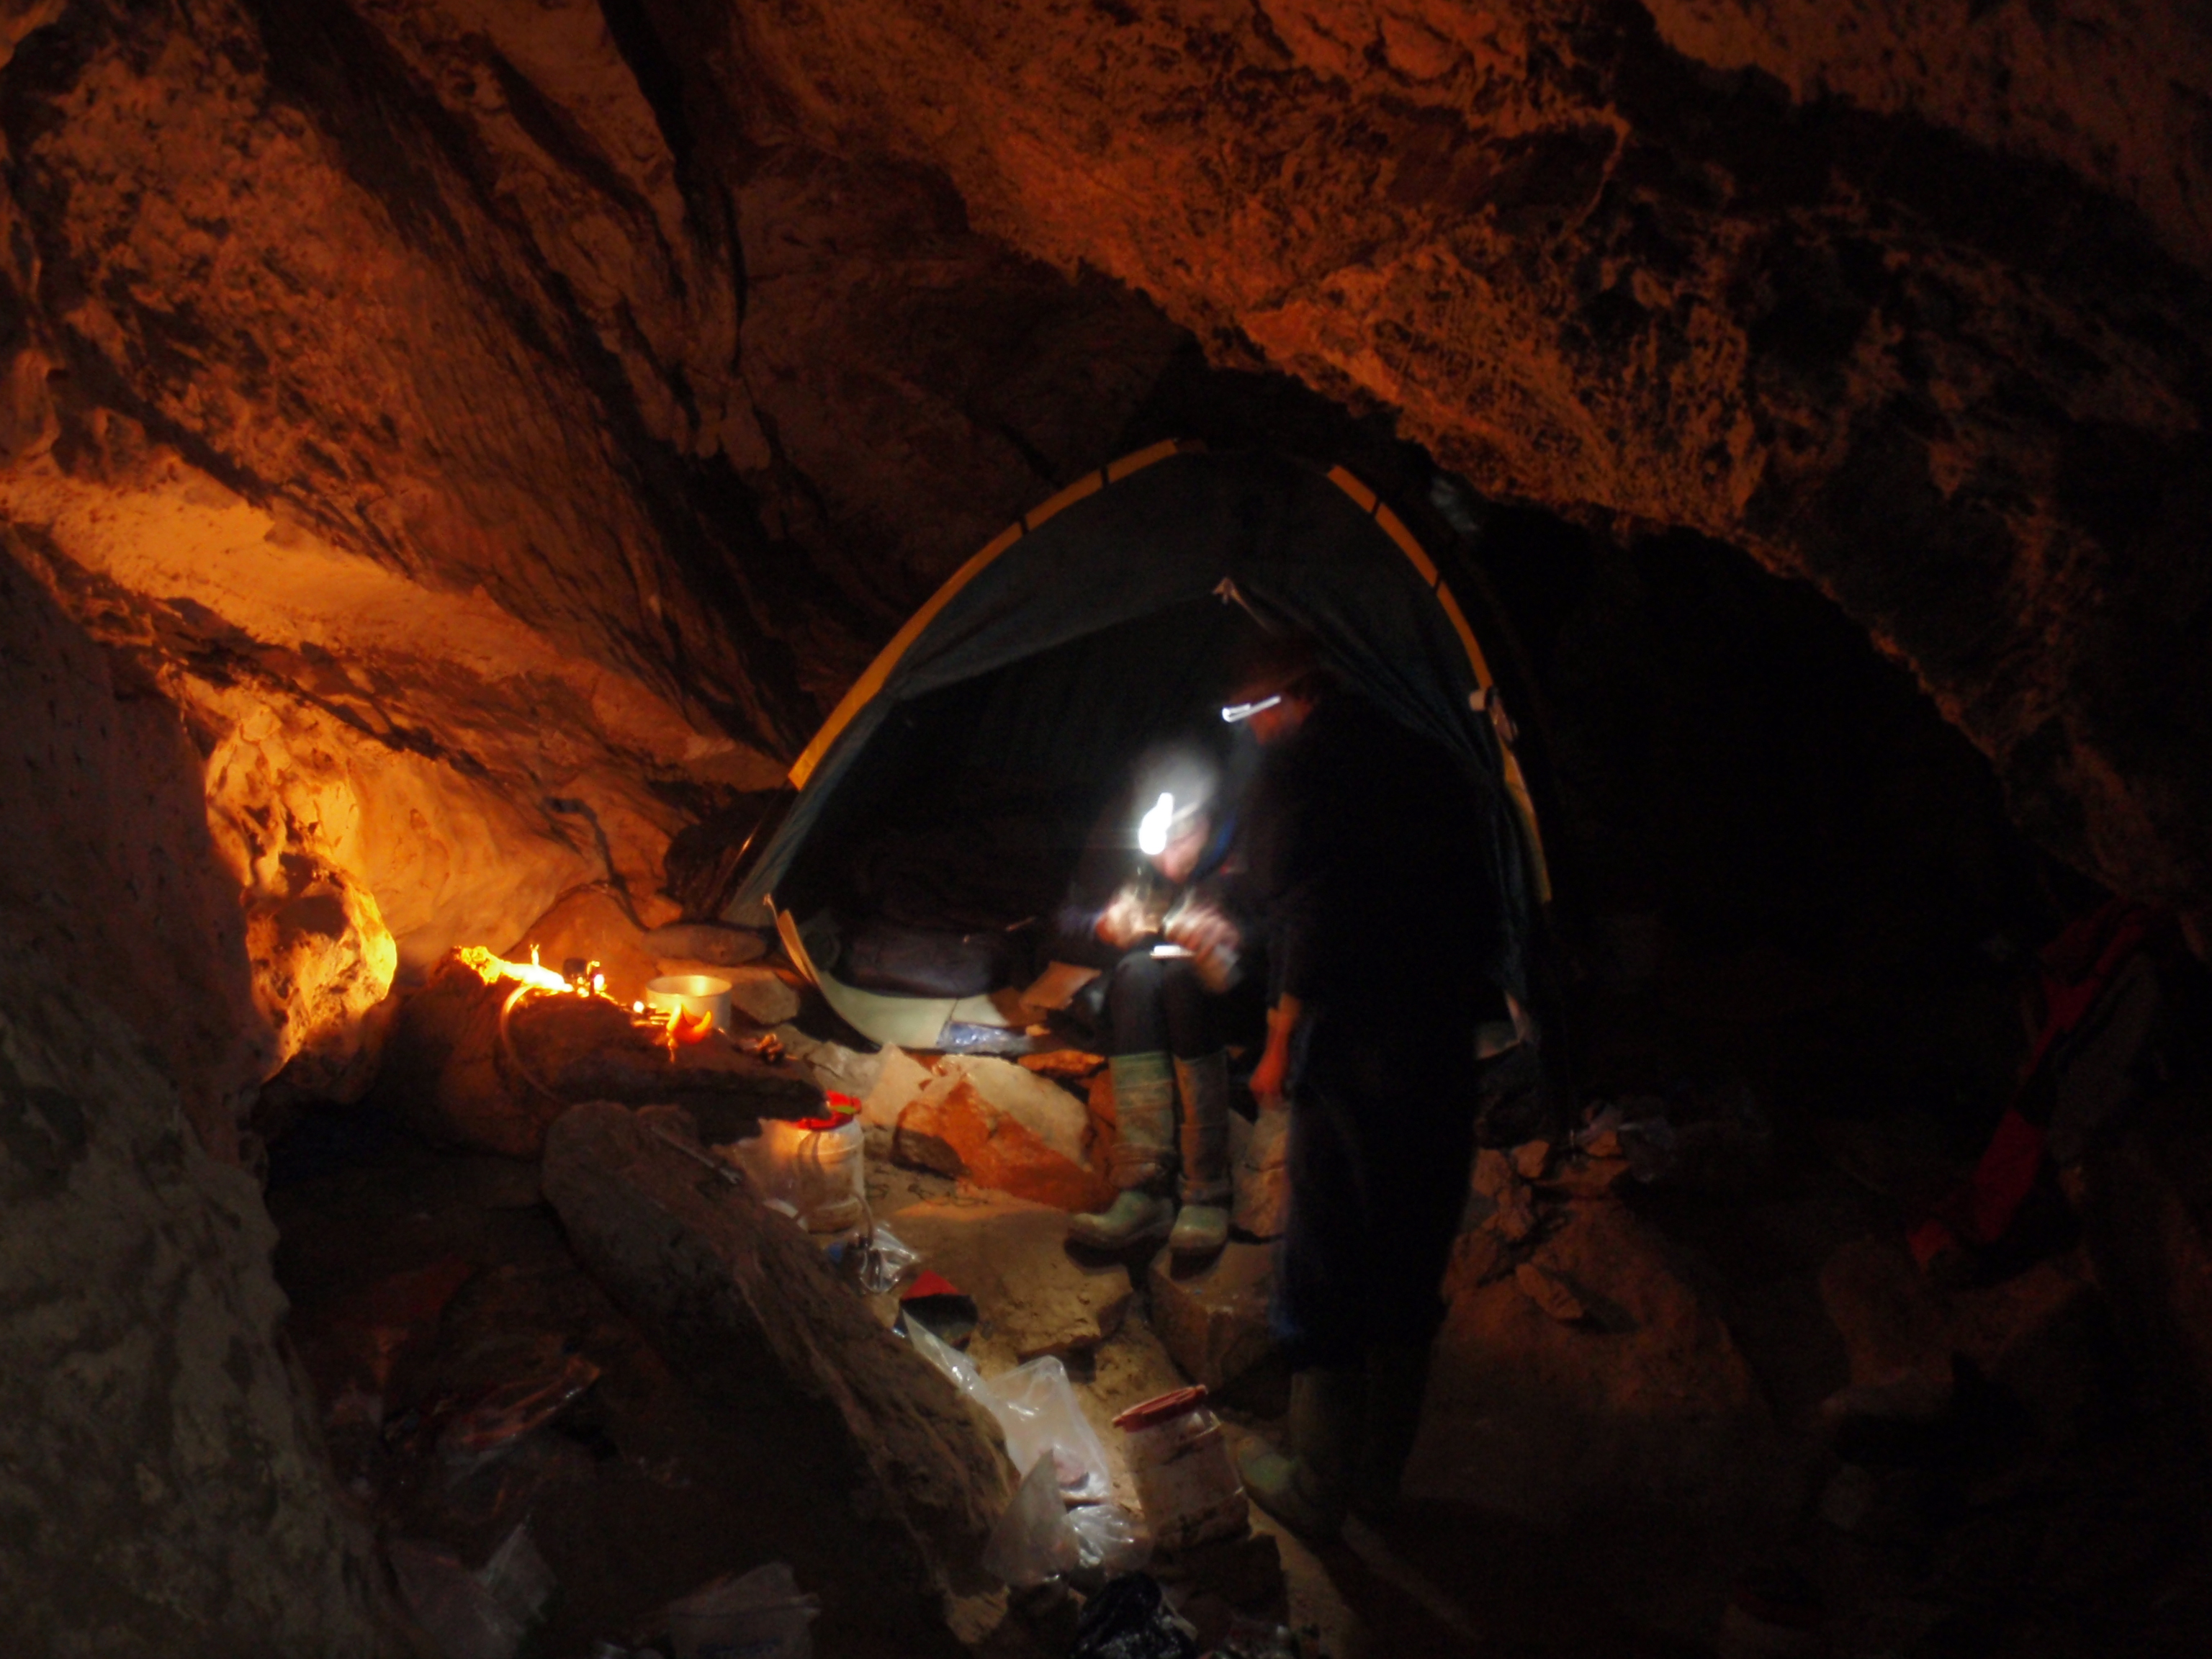
\includegraphics[width=\linewidth]{2010/povodni/20100729-13-13-11 - Iztok Mozir - P7294694 - Camp X-ray--orig.jpg}}
\caption{The ambience of camp \protect\passage{X-ray}. \pic{Iztok Možir}}
\end{figure*}

\tweet{2:24PM Aug 7th, 2010}{
Latest round of camps:now 2km of new cave,all found deeper than 500m.Korita finished\&derigged,final effort on pitch series off PrinceCon\ldots{}}